\section{Background: Storage Strategies in PyPy}



\subsection{Static Objects}
\label{cha:staticObjects}

\todo{Removed this section?}

The most important optimization implemented by RPythons tracing JIT is an aggressive escape analysis \cite{escapeAnalysis}.
The escape analysis is conducted using a form of partial evaluation \cite{allocRemJIT}.
In short, it works by traversing the original trace, replacing object allocations with \emph{static objects}, and turning a static object back to a normal allocation when it is observed to escape the trace.
A static object is allocated directly on the stack, effectively avoiding the heap allocation.
This optimization is safe because the optimizer can prove that static objects don't affect the program state after the program exits the loop.

For an example, consider the \lstinline{SmallInteger} objects created inside the loop in listing \ref{lst:TraceExample1} on page \pageref{lst:TraceExample1}.
These \lstinline{SmallInteger} objects are not escaping the loop, because the only reference to each object is deleted at the end of each iteration.
Only the object allocated in the very last iteration persists after the loop ends.
Thus, all intermediate \lstinline{SmallInteger} instances don't need to be allocated; they are treated as static objects.
Their content is maintained on the stack instead of the heap, potentially even optimized into machine registers.

The drawback of static objects is a rather complex deoptimization.
As mentioned above, an optimized JIT trace must be left when a guard check, inserted to ensure correctness of the code, fails.
In such a case the escape analysis performed as basis for the static object optimization does not hold anymore.
Static objects allocated in the last loop iteration have to be allocated on the heap, and their contents have to be copied from the stack to the newly allocated objects.
To do this, the JIT has to maintain information about the stack layout while executing an optimized trace; using a stack map, the stack can be walked in order to create non-static versions of the objects.

Since RPythons meta tracing JIT creates traces of VM operations, not only language level objects can be turned into static objects, but also VM level objects.
Just like other optimizations in the RPython toolchain, this leads to cleaner code; short living objects can substantially increase the expressiveness of VM code.


\subsection{Storage Strategies}
\label{cha:storageStrategies}

Usually, collections in dynamic languages are represented by allocating an array and filling it with pointers that point to the actual elements of the collection.
This is because in a dynamic language, or even any language with polymorphism, objects of different types can be added to the same collection.
Using an array of pointers is the generic way to represent such a dynamic collection.
However, it also introduces an indirection between the collection and the actual elements.
To access any value from the collection, the VM must first fetch the pointer address and dereference it, before fetching the actual value.
This additional memory access is a big overhead compared to a C array of pure integer values, that a program can traverse in full speed.

Another allocation removal technique called storage strategies, or strategies for short, can optimize dynamic collections \cite{strategies}.
Storage strategies are implemented on VM level and are based on the idea that the VM has multiple possible ways of representing every collection internally.
Based on the user program and the operations performed on a collection, the VM can switch between multiple strategies and choose the most efficient one.
To do so, the collection contains a reference to the currently used strategy object, and all important operations performed on the collection are delegated to that object.
Ideally the strategy will not be switched very often, so the second important idea behind storage strategies is that user programs often utilize collections in a predictable way.

For example, collections are often used in a homogeneous way.
If the first few elements appended to a Python list are integers, then it is likely that the user program will keep storing only integer values in that list.
This is enough information to optimize the list.
In this case, the VM could allocate an array for integer values and store the values directly, without allocating box objects to represent these integers.
Figure \ref{fig:IntegerStorage} illustrates this example by showing two possible representations for the same collection: the collection on the left side contains boxed integer objects, while the collection on the right side contains pure integer values.

\begin{figure}[ht]
\centering
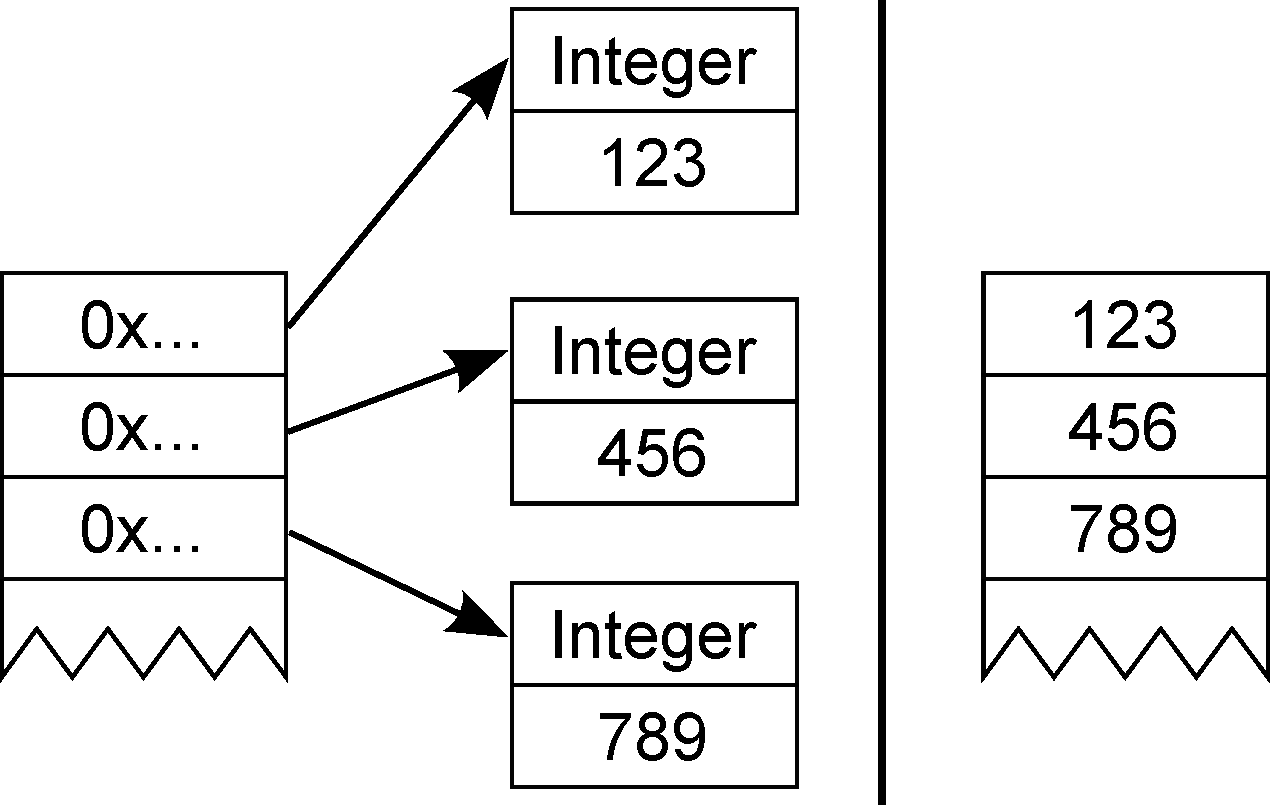
\includegraphics[width=0.4\textwidth]{strategies_intStorage}
\caption{Example for a storage strategy}
\label{fig:IntegerStorage}
\small
Left side: generic collection holding only boxed integer objects.\\
Right size: Optimized collection, resulting in less object allocations and memory usage.
\end{figure}

In order to optimize the internal representation of a collection, the VM must make assumptions about the usage pattern of that collection.
It cannot wait until a collection has been used for a while before optimizing it, otherwise it might end up not optimizing short living or small collections.
Optimizing short living collections can be very important, for example when they are allocated frequently in a tight loop.
In order to optimize as many collections as possible, the VM must predict the usage pattern based on the very first operations performed on a collection.

Making predictions about usage patterns is hard and the success can vary depending on the situation.
Therefore, the VM should make assumptions based on meaningful heuristics, which can be obtained by examining existing systems and deriving typical usage patterns.
But even with these preconditions there will be cases where the VMs assumptions turn out to be wrong.
In such cases, the VM must uphold the semantics of the programming language and perform a \emph{deoptimization}.
Most of the time this means allocating a new, more general collection and copying all elements from the old collection into the new one.
Figure \ref{fig:Deoptimization} shows an example of this procedure.
The storage on the left is optimized to hold integer values, but the user program wants to add a float value to the list.
The VM has to allocate a new, more general storage array which is able to hold generic objects.
In this case, the deoptimization could have been avoided if the VM had implemented a storage strategy to hold both integer and float values.
The deoptimization procedure must be tuned for highest performance, and should take place as rarely as possible.

\begin{figure}[ht]
\centering
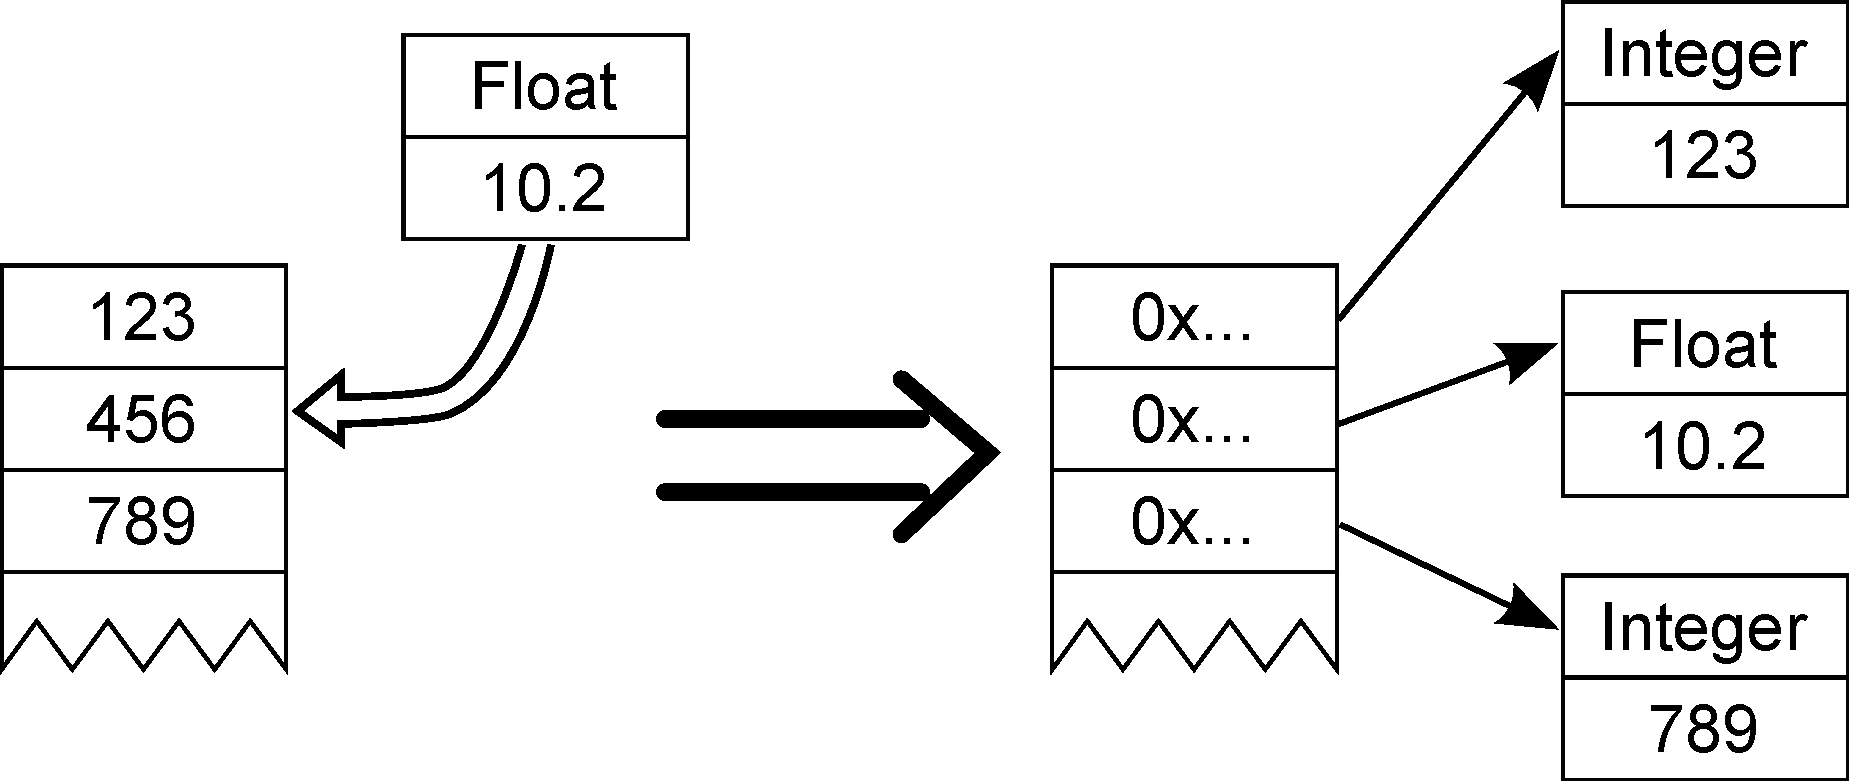
\includegraphics[width=0.4\textwidth]{strategies_deoptimization}
\caption{Deoptimization of an optimized integer collection}
\label{fig:Deoptimization}
\small
A general storage array has to be created, and Integer objects have to be allocated.
\end{figure}

\subsubsection{Homogeneous Collections}

As indicated by the examples in the previous section, the most important optimization target of storage strategies are homogeneous collections.
A collection is homogeneous when it only contains elements of a single type.
Since the size of the datatype is known, the VM can allocate an array big enough to hold the data of many such objects in consecutive memory.
The benefit of this optimization is two-fold: the VM can save the memory for the objects, and accessing the objects becomes faster due to the missing indirection between collection and elements.

This optimization is not limited to numeric datatypes like integers.
Even objects with multiple fields can be represented that way, as illustrated in figure \ref{fig:MultipleInlinedFields}.
The fields of each objects just have to be placed in memory in sequence.
Accessing any field in any object can happen without additional memory access, simply based on constant-time pointer arithmetics.

\begin{figure}[ht]
\centering
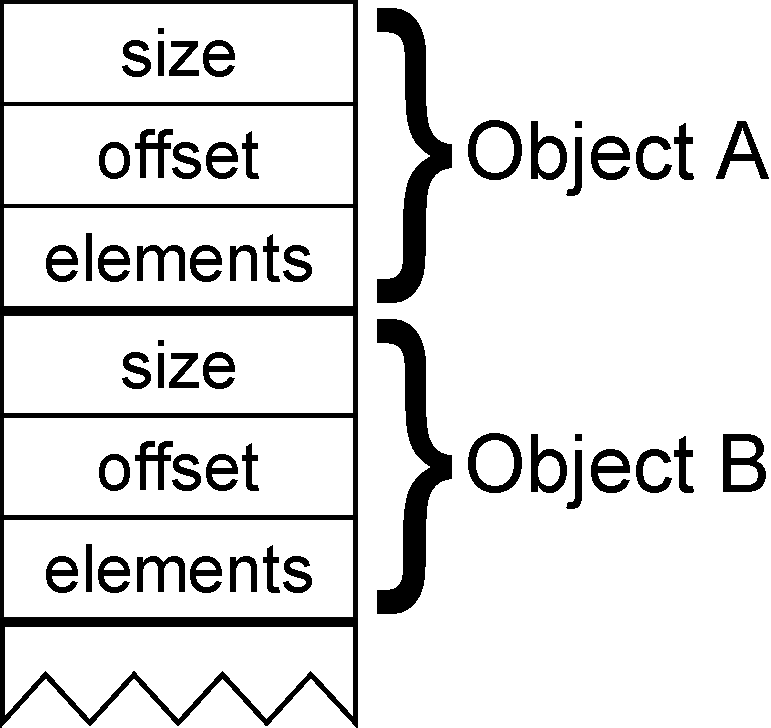
\includegraphics[width=0.27\textwidth]{strategies_multipleFields}
\caption{Inlining storage for composite objects with 3 fields}
\label{fig:MultipleInlinedFields}
\end{figure}
